\begin{frame}{Two questions for the R laboratory}
\begin{itemize}
\item How does the sample mean vary across repeated samples? Municipal pension income, with sample sizes 10, 100 and 1,000.
\item How do we analyse a relationship between two variables? BES education indicators, tables, groups and quantitative pairs.
\end{itemize}
\par\vspace{4mm}\href{https://silviasaliniunimi.github.io/data-analysis-tax-compliance/05-r-laboratory.html}{Open the laboratory guide and download the complete R project}
\end{frame}

\begin{frame}[fragile]{The RStudio project}
Extract the project and open \texttt{HCAI\_R\_Lab.Rproj}.\begin{lstlisting}[language=R]
getwd()
list.files("data")
source("scripts/01_sampling_mean.R")
source("scripts/02_bivariate.R")
\end{lstlisting}
Run selected lines with Ctrl+Enter, or Cmd+Enter on a Mac. Both scripts use base R. Results appear in \texttt{results/}.
\end{frame}

\begin{frame}{Part A: sampling distributions}
\Large The observations vary across municipalities.\\[4mm]The estimate varies across samples.\par\vspace{6mm}\normalsize\href{https://silviasaliniunimi.github.io/data-analysis-tax-compliance/03-inference.html}{Revisit the inference e-tivity}
\end{frame}

\begin{frame}[fragile]{The municipal income file}
The supplied teaching snapshot contains \textbf{8,047 municipalities}.\begin{lstlisting}[language=R]
municipalities <- read.csv("data/redditi.csv",
  check.names = FALSE,
  colClasses = c(Cod = "character"))
nrow(municipalities)
head(municipalities)
\end{lstlisting}
\texttt{Rp\_avg}: municipal pension-income average, in EUR.\\\texttt{Rp\_share}: pension income / taxable income, as a percentage.
\end{frame}

\begin{frame}[fragile]{The target determines the mean}
\begin{lstlisting}[language=R]
mean(municipalities$Rp_avg)
# 14366.97 EUR
sum(municipalities$Rp_tot) /
  sum(municipalities$Rp_freq)
# 16703.62 EUR
\end{lstlisting}
The first gives each municipality the same weight. The second weights municipal means by pension-income frequency.\prompt{Which quantity describes the typical municipality? Which uses the aggregate amount and frequency?}
\end{frame}

\begin{frame}[fragile]{One random sample}
\begin{lstlisting}[language=R]
set.seed(1111)
N <- nrow(municipalities)
n <- 100
selected <- sample.int(N, n, replace = FALSE)
one_sample <- municipalities[selected, ]
mean(one_sample$Rp_avg)
# 14309.60 EUR
\end{lstlisting}
Sampling error: $14,309.60-14,366.97=-57.37$ EUR. The seed reproduces this particular draw.
\end{frame}

\begin{frame}{Sample size and repetitions}
\begin{tabular}{lp{.69\textwidth}}\toprule
$N=8047$ & Municipalities in the finite teaching population\\[4mm]
$n=10,100,1000$ & Municipalities in one sample\\[4mm]
$B=200$ & Independent repetitions of the complete sampling experiment\\\bottomrule
\end{tabular}\par\vspace{4mm}A municipality appears at most once within a sample. It can reappear in another replicate.
\prompt{Increasing $B$ describes the sampling distribution more accurately. Does it change the uncertainty of one sample of size $n$?}
\end{frame}

\begin{frame}[fragile]{Repeated samples in R}
\begin{lstlisting}[language=R]
set.seed(20261111)
B <- 200
n <- 10
means_n10 <- replicate(B, {
  selected <- sample.int(N, n, replace = FALSE)
  mean(municipalities$Rp_avg[selected])
})
mean(means_n10)
sd(means_n10)
\end{lstlisting}
The supplied script repeats the calculation for both variables and all three sample sizes.
\end{frame}

\begin{frame}{Population and means from small samples}
\centering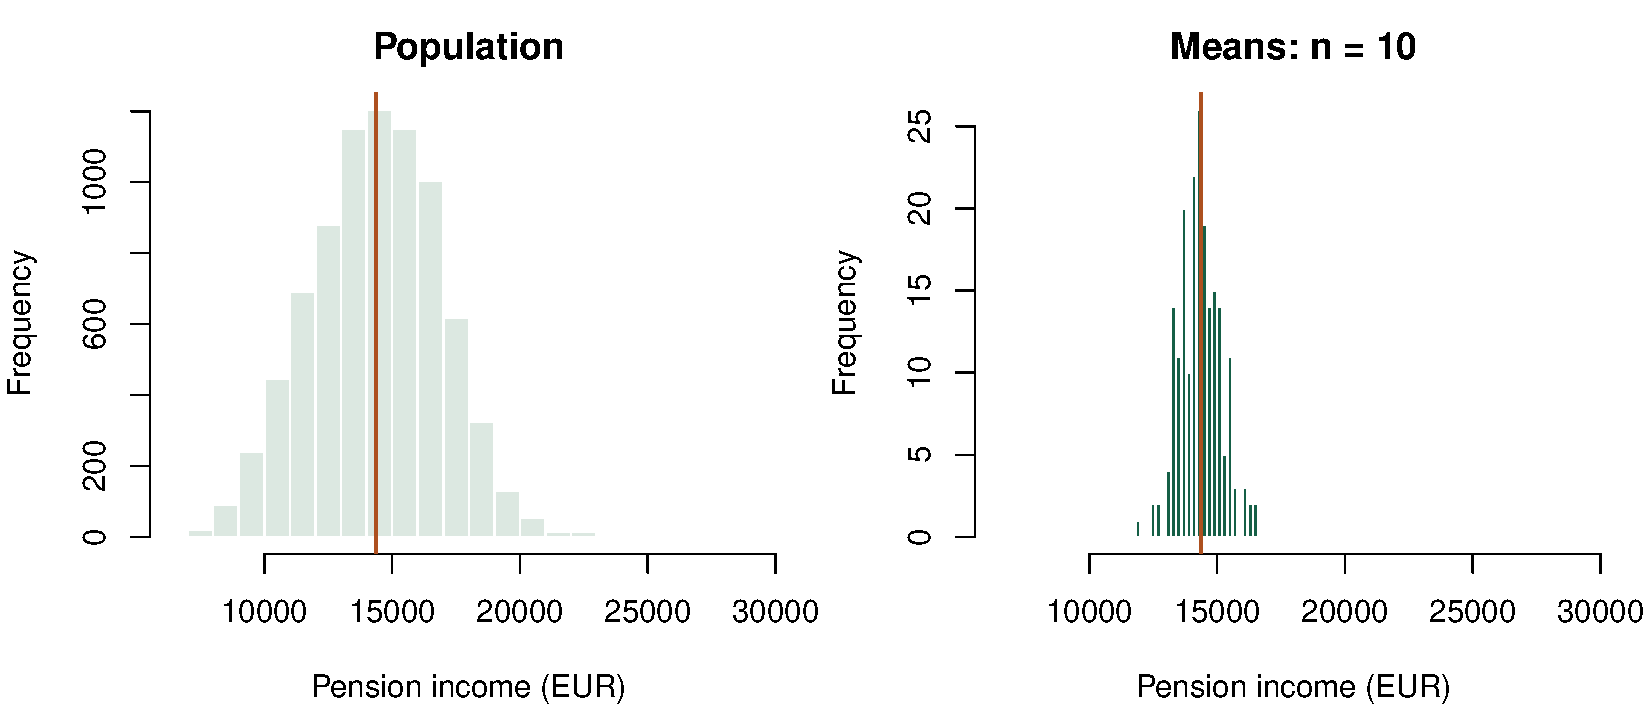
\includegraphics[width=.98\textwidth,height=.63\textheight,keepaspectratio]{figures/r-lab/sampling_pair_1.pdf}
\par\small Both panels use the same horizontal range. The right panel contains means of whole samples.
\end{frame}

\begin{frame}{Means from larger samples}
\centering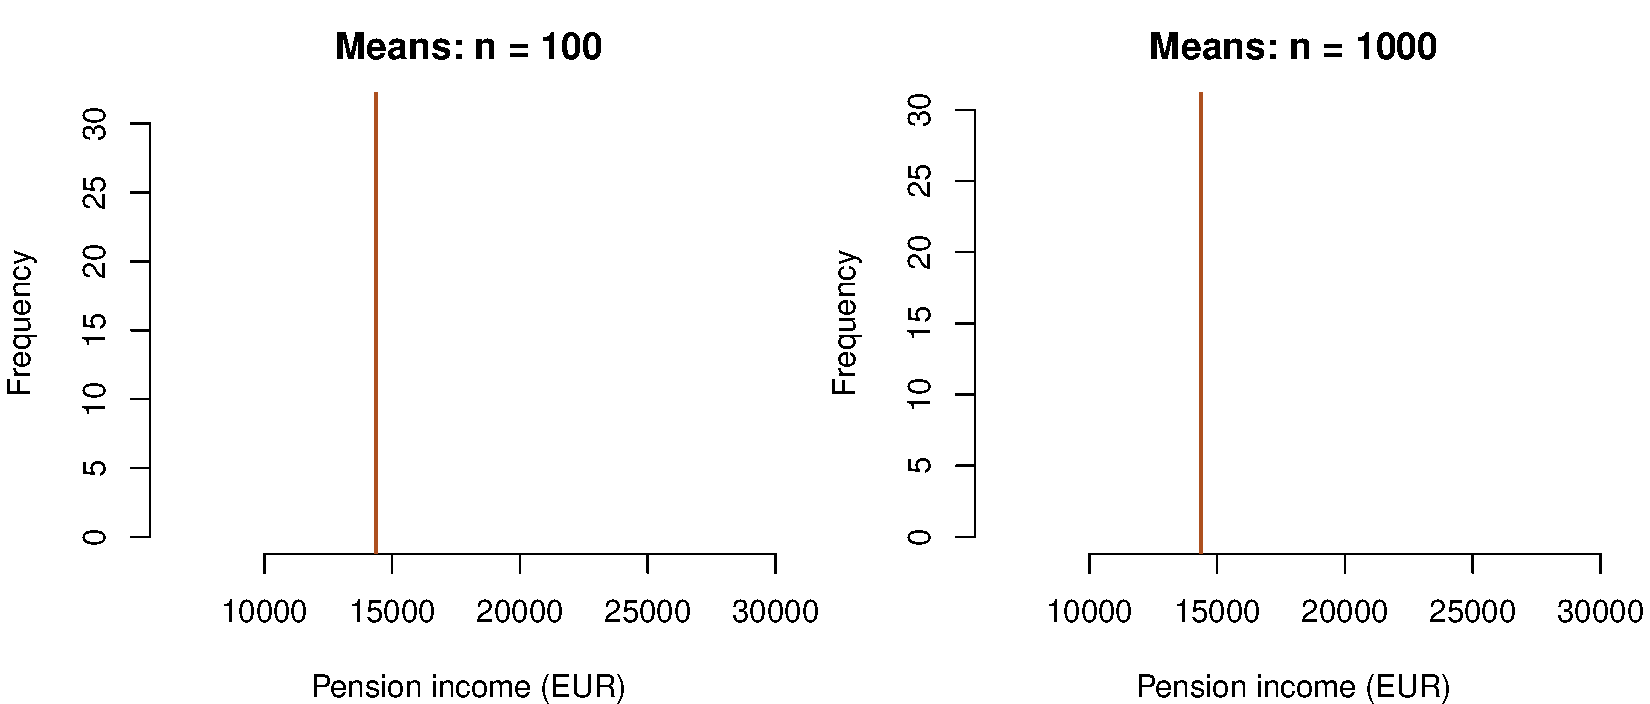
\includegraphics[width=.98\textwidth,height=.63\textheight,keepaspectratio]{figures/r-lab/sampling_pair_2.pdf}
\par\small The scale is unchanged. Larger samples make the distribution of the mean more concentrated.
\end{frame}

\begin{frame}{The standard error under this design}
Use the finite-population variance with denominator $N-1$:
\[S^2=\frac{1}{N-1}\sum_{i=1}^N(y_i-\mu)^2.\]
For simple random sampling without replacement,
\[\operatorname{SE}(\bar Y)=\sqrt{\frac{1-n/N}{n}S^2}.\]
Larger $n$ reduces the spread of the estimator. At $n=N$, the supplied population mean is known exactly.
\end{frame}

\begin{frame}{Empirical and theoretical standard errors}
\begin{center}\begin{tabular}{rrrr}\toprule
$n$ & Mean of 200 means & Empirical SE & Theoretical SE\\\midrule
10 & 14,347.04 & 788.94 & 800.59\\[2mm]
100 & 14,384.03 & 264.75 & 251.75\\[2mm]
1,000 & 14,367.89 & 72.64 & 74.97\\\bottomrule\end{tabular}\end{center}
All values are in EUR. The target is $14,366.97$ EUR.
\prompt{Why do empirical and theoretical values differ? What would increasing $B$ change?}
\end{frame}

\begin{frame}{Two sample means at once}
\centering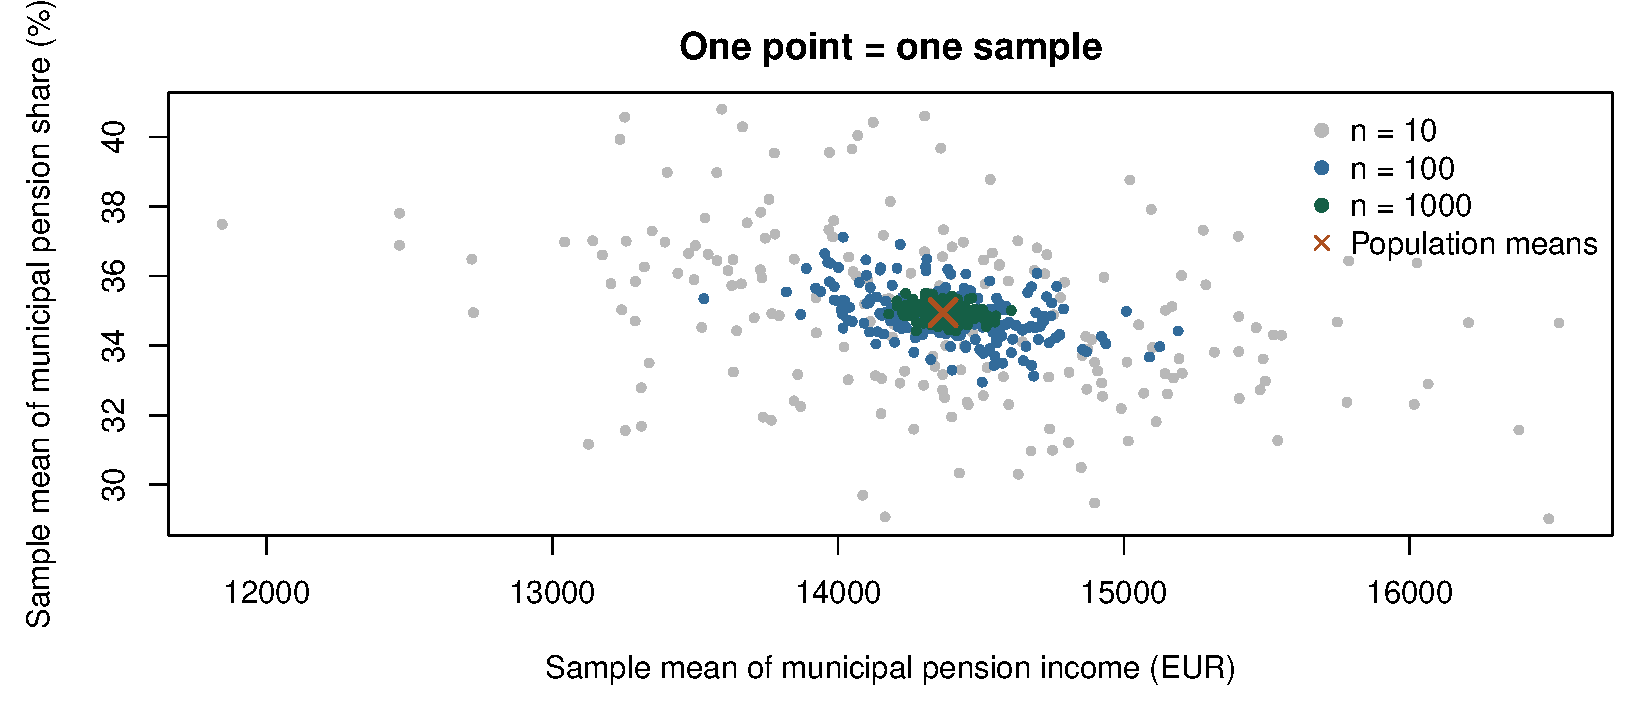
\includegraphics[width=.98\textwidth,height=.63\textheight,keepaspectratio]{figures/r-lab/two_sample_means.pdf}
\par\small Each point summarises one sample. Larger samples concentrate near the pair of population means.
\end{frame}

\begin{frame}{A restricted sampling frame}
An optional simulation samples 100 municipalities only from the highest-income quarter.
\begin{center}\begin{tabular}{lr}\toprule
Target mean, all supplied municipalities & 14,366.97 EUR\\[2mm]
Mean of the restricted-frame estimates & 17,548.66 EUR\\[2mm]
SD of the restricted-frame estimates & 127.60 EUR\\\bottomrule\end{tabular}\end{center}
The procedure estimates a different frame mean with considerable precision.
\prompt{How could we change the design to address the original target?}
\end{frame}

\begin{frame}{Part A: interpretation exercise}
Change the number of repetitions to 2,000, keeping the sample sizes fixed.
\begin{itemize}
\item Compare the means and empirical standard errors with the reference table.
\item Explain the different roles of $n$ and $B$.
\item State the unit of analysis and target population.
\item Explain why the population observations need not become normally distributed.
\end{itemize}

\end{frame}

\begin{frame}{Part B: bivariate analysis}
\Large The question and the two variable types determine the method.\par\vspace{6mm}\normalsize\href{https://silviasaliniunimi.github.io/data-analysis-tax-compliance/04-bivariate.html}{Revisit the bivariate e-tivity}
\end{frame}

\begin{frame}[fragile]{The BES education file}
\begin{lstlisting}[language=R]
bes <- read.csv("data/bes_education.csv")
nrow(bes)
# 20
names(bes)
table(bes$area)
\end{lstlisting}
One row represents a region. We retain Trentino-Alto Adige and exclude its two autonomous provinces to avoid overlapping observations.
\end{frame}

\begin{frame}{Questions and methods}
\small\begin{tabular}{p{.43\textwidth}p{.46\textwidth}}\toprule
\textbf{Question} & \textbf{Starting point}\\\midrule
Area and high early leaving & Contingency table, conditional proportions, association\\[3mm]
NEET across two dropout groups & Group distributions and Welch's t test\\[3mm]
NEET across four areas & Group distributions and one-way ANOVA\\[3mm]
Culture and tertiary education & Scatterplot and Pearson correlation\\\bottomrule\end{tabular}
\end{frame}

\begin{frame}[fragile]{A categorical variable from a threshold}
\begin{lstlisting}[language=R]
bes$dropout <- factor(
  ifelse(bes$early_leaving_pct > 15,
         "Above 15%", "At most 15%"),
  levels = c("At most 15%", "Above 15%"))
tab <- table(bes$area, bes$dropout)
prop.table(tab, margin = 1) * 100
\end{lstlisting}
The threshold defines the comparison before the test. It discards differences within each category.
\end{frame}

\begin{frame}{Counts and conditional percentages}
\begin{center}\begin{tabular}{lrrr}\toprule
Area & At most 15\% & Above 15\% & Total\\\midrule
North-West & 4 & 0 & 4\\
North-East & 4 & 0 & 4\\
Centre & 4 & 0 & 4\\
South-Islands & 4 & 4 & 8\\\midrule
Total & 16 & 4 & 20\\\bottomrule\end{tabular}\end{center}
Within South-Islands, 50\% of regions exceed the threshold. All four above-threshold regions belong to South-Islands.
\prompt{State the denominator in each sentence.}
\end{frame}

\begin{frame}[fragile]{Expected counts before a p-value}
\begin{lstlisting}[language=R]
chi <- suppressWarnings(chisq.test(tab,
                                  correct = FALSE))
chi$expected
sum(chi$expected < 5)
# 7 of 8 cells
fisher.test(tab)
# p-value = 0.07699
\end{lstlisting}
Here $\chi^2=7.5$ and Cram\'{e}r\textquotesingle s $V=0.6124$. Sparse expected counts undermine the asymptotic approximation.
\end{frame}

\begin{frame}{Exact tests and the inferential model}
\begin{itemize}
\item Fisher's test conditions on the observed margins under its sampling model.
\item It addresses sparse counts in this comparison.
\item It does not establish independence of neighbouring regions or remove confounding.
\item These 20 regions form the observed territorial set. Inference requires a model beyond describing that set.
\end{itemize}
\prompt{What can we state directly from the table before choosing an inferential model?}
\end{frame}

\begin{frame}{NEET percentages across groups}
\centering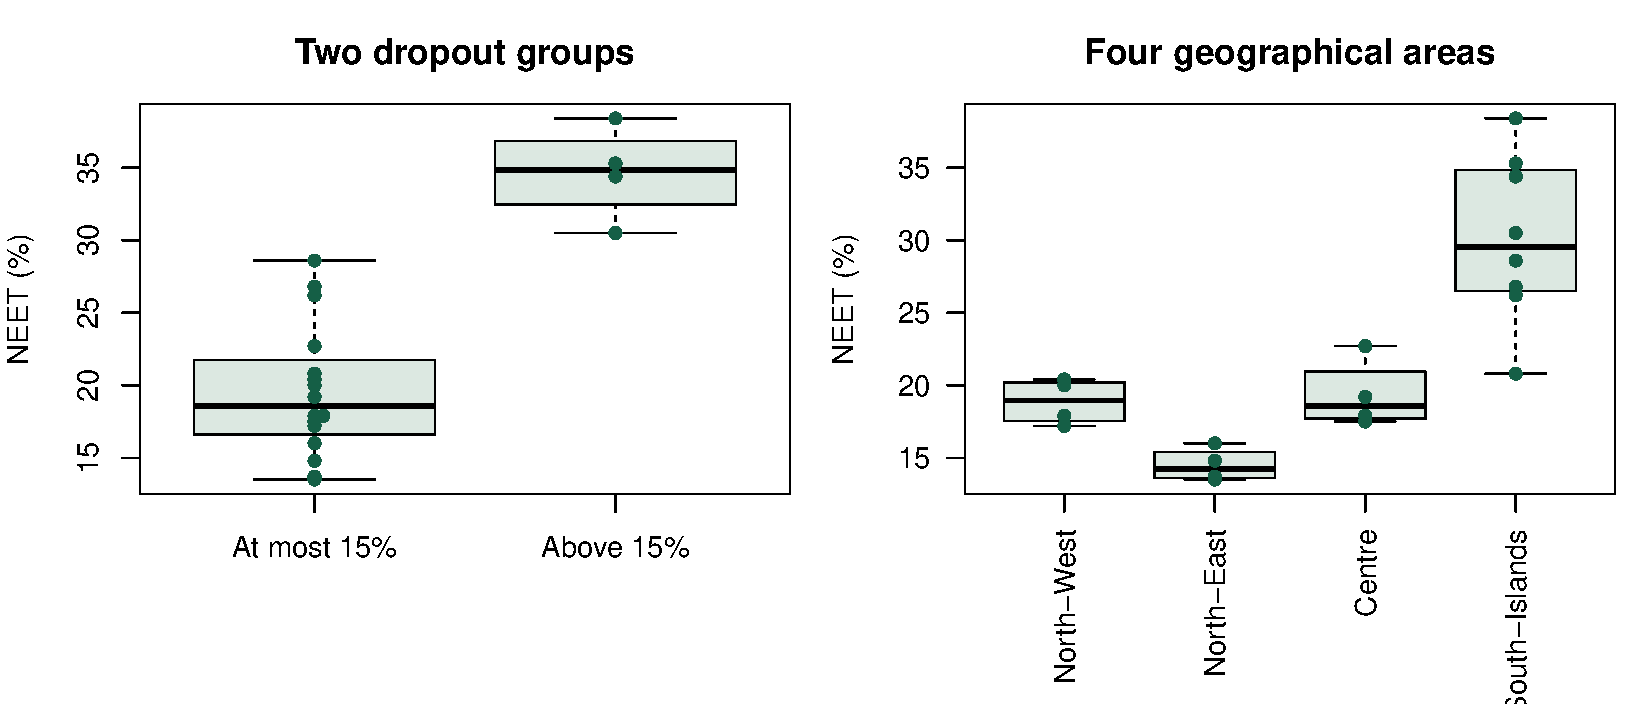
\includegraphics[width=.98\textwidth,height=.63\textheight,keepaspectratio]{figures/r-lab/group_comparisons.pdf}
\par\small Each dot is one region. Mean NEET is 34.65\% in the four above-threshold regions and 19.575\% in the other sixteen.
\end{frame}

\begin{frame}[fragile]{Two groups: Welch's t test}
\begin{lstlisting}[language=R]
t.test(neet_pct ~ dropout, data = bes)
\end{lstlisting}
\begin{center}\begin{tabular}{lr}\toprule
Mean difference, group 1 minus group 2 & $-15.075$ percentage points\\
$t$ and degrees of freedom & $-7.586$, $6.367$\\
95\% interval for the difference & $[-19.870,-10.280]$\\
Two-sided model-based p-value & $0.000205$\\\bottomrule\end{tabular}\end{center}
Group order: \emph{At most 15\%} minus \emph{Above 15\%}. Inference relies on the comparison model and independent observations.
\end{frame}

\begin{frame}[fragile]{Several groups: one-way ANOVA}
\begin{lstlisting}[language=R]
fit_anova <- aov(neet_pct ~ area, data = bes)
summary(fit_anova)
\end{lstlisting}
\[F(3,16)=16.856,\quad p=0.0000330,\quad \eta^2=0.7596.\]\begin{itemize}
\item The global alternative says at least one model mean differs.
\item Classical ANOVA assumes independent, normal errors with a common variance.
\item Inspect the small groups and consider unequal-variance methods.
\end{itemize}

\end{frame}

\begin{frame}[fragile]{Two quantitative variables}
\begin{lstlisting}[language=R]
plot(tertiary_pct ~ cultural_pct, data = bes)
cor(bes$cultural_pct, bes$tertiary_pct)
# 0.7277
cor(bes[c("tertiary_pct", "cultural_pct",
          "reading_pct", "library_pct")])
\end{lstlisting}
The percentages describe regional aggregates. Correlation measures the linear relationship between those regional values.
\end{frame}

\begin{frame}{Cultural participation and tertiary education}
\centering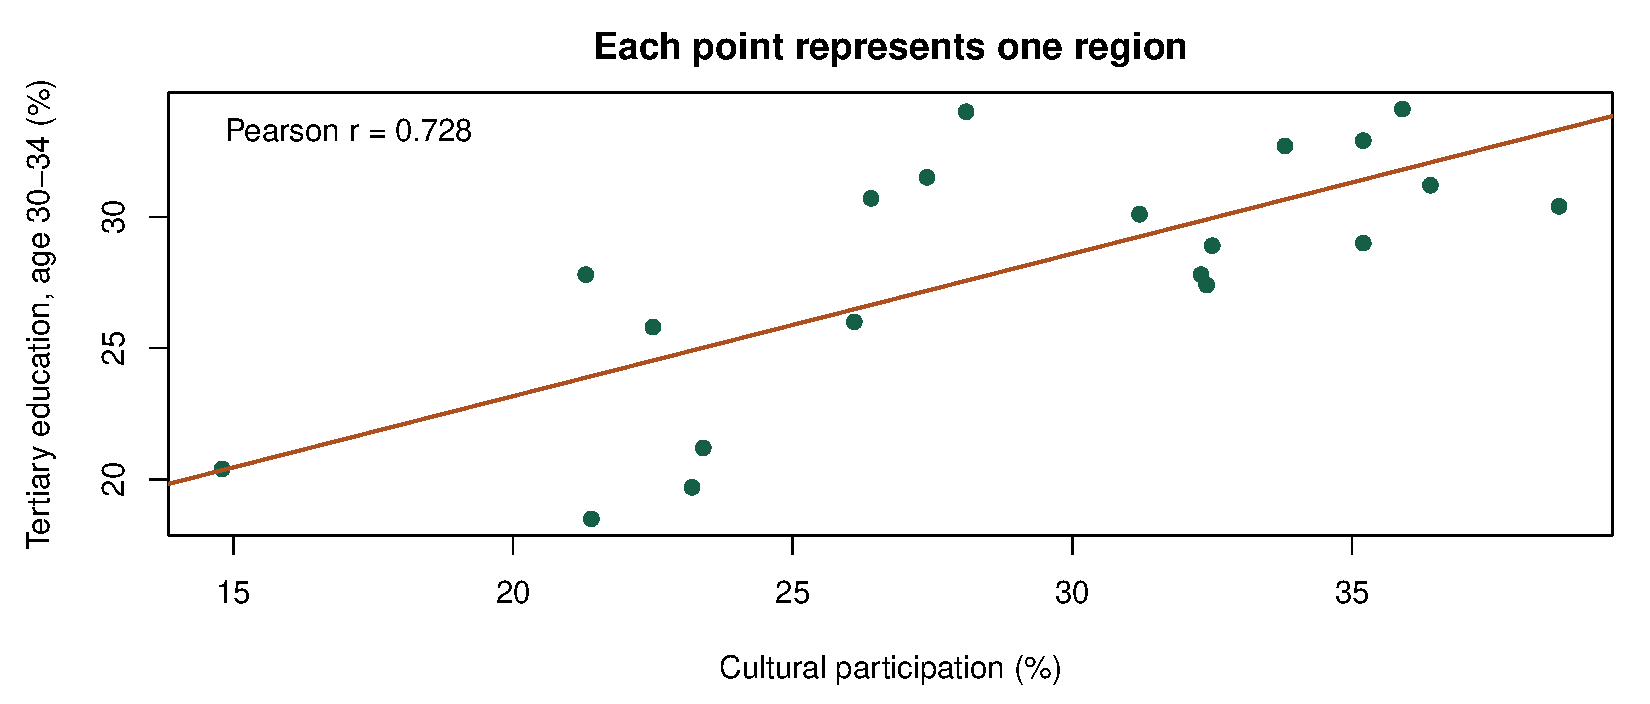
\includegraphics[width=.98\textwidth,height=.63\textheight,keepaspectratio]{figures/r-lab/correlation.pdf}
\par\small The positive regional association does not identify an individual effect or a causal mechanism.
\end{frame}

\begin{frame}[fragile]{Optional bridge: a fitted line}
\begin{lstlisting}[language=R]
fit_line <- lm(tertiary_pct ~ cultural_pct,
               data = bes)
summary(fit_line)
\end{lstlisting}
\[\widehat{\text{tertiary percentage}}=12.323+0.5424\times\text{cultural percentage}.\]\[R^2=0.5296.\]A one-percentage-point difference in cultural participation is associated with about 0.542 percentage points in the fitted response. Predictive evaluation follows in supervised learning.
\end{frame}

\begin{frame}{Part B: a short analytical report}
\begin{itemize}
\item State the unit, variables and comparison.
\item Report a descriptive effect in meaningful units.
\item Explain the conditions behind any test you report.
\item Distinguish regional association from a causal or individual claim.
\end{itemize}
\par\vspace{3mm}\href{https://silviasaliniunimi.github.io/data-analysis-tax-compliance/05-r-laboratory.html}{Laboratory guide, scripts and data dictionary}
\end{frame}
